Si en lugar de 100 presos se consideran n, donde n es un número natural arbitrario, la probabilidad de supervivencia de los prisioneros con la estrategia de seguimiento del ciclo está dada por la ecuación \ref{eq:prob_supervivencia_n}

\begin{equation}\label{eq:prob_supervivencia_n}
    1-(H_2n-H_n)=1-(H_2n-\ln 2n)+(H_n-\ln n) -\ln 2
\end{equation}

y con n $\to$ infinito
\begin{equation}\label{eq:prob_supervivencia_n_infinito}
lim_{n \to \infty} (H_n-\ln n)=\gamma
\end{equation}

\begin{figure}[H]
    \centering
    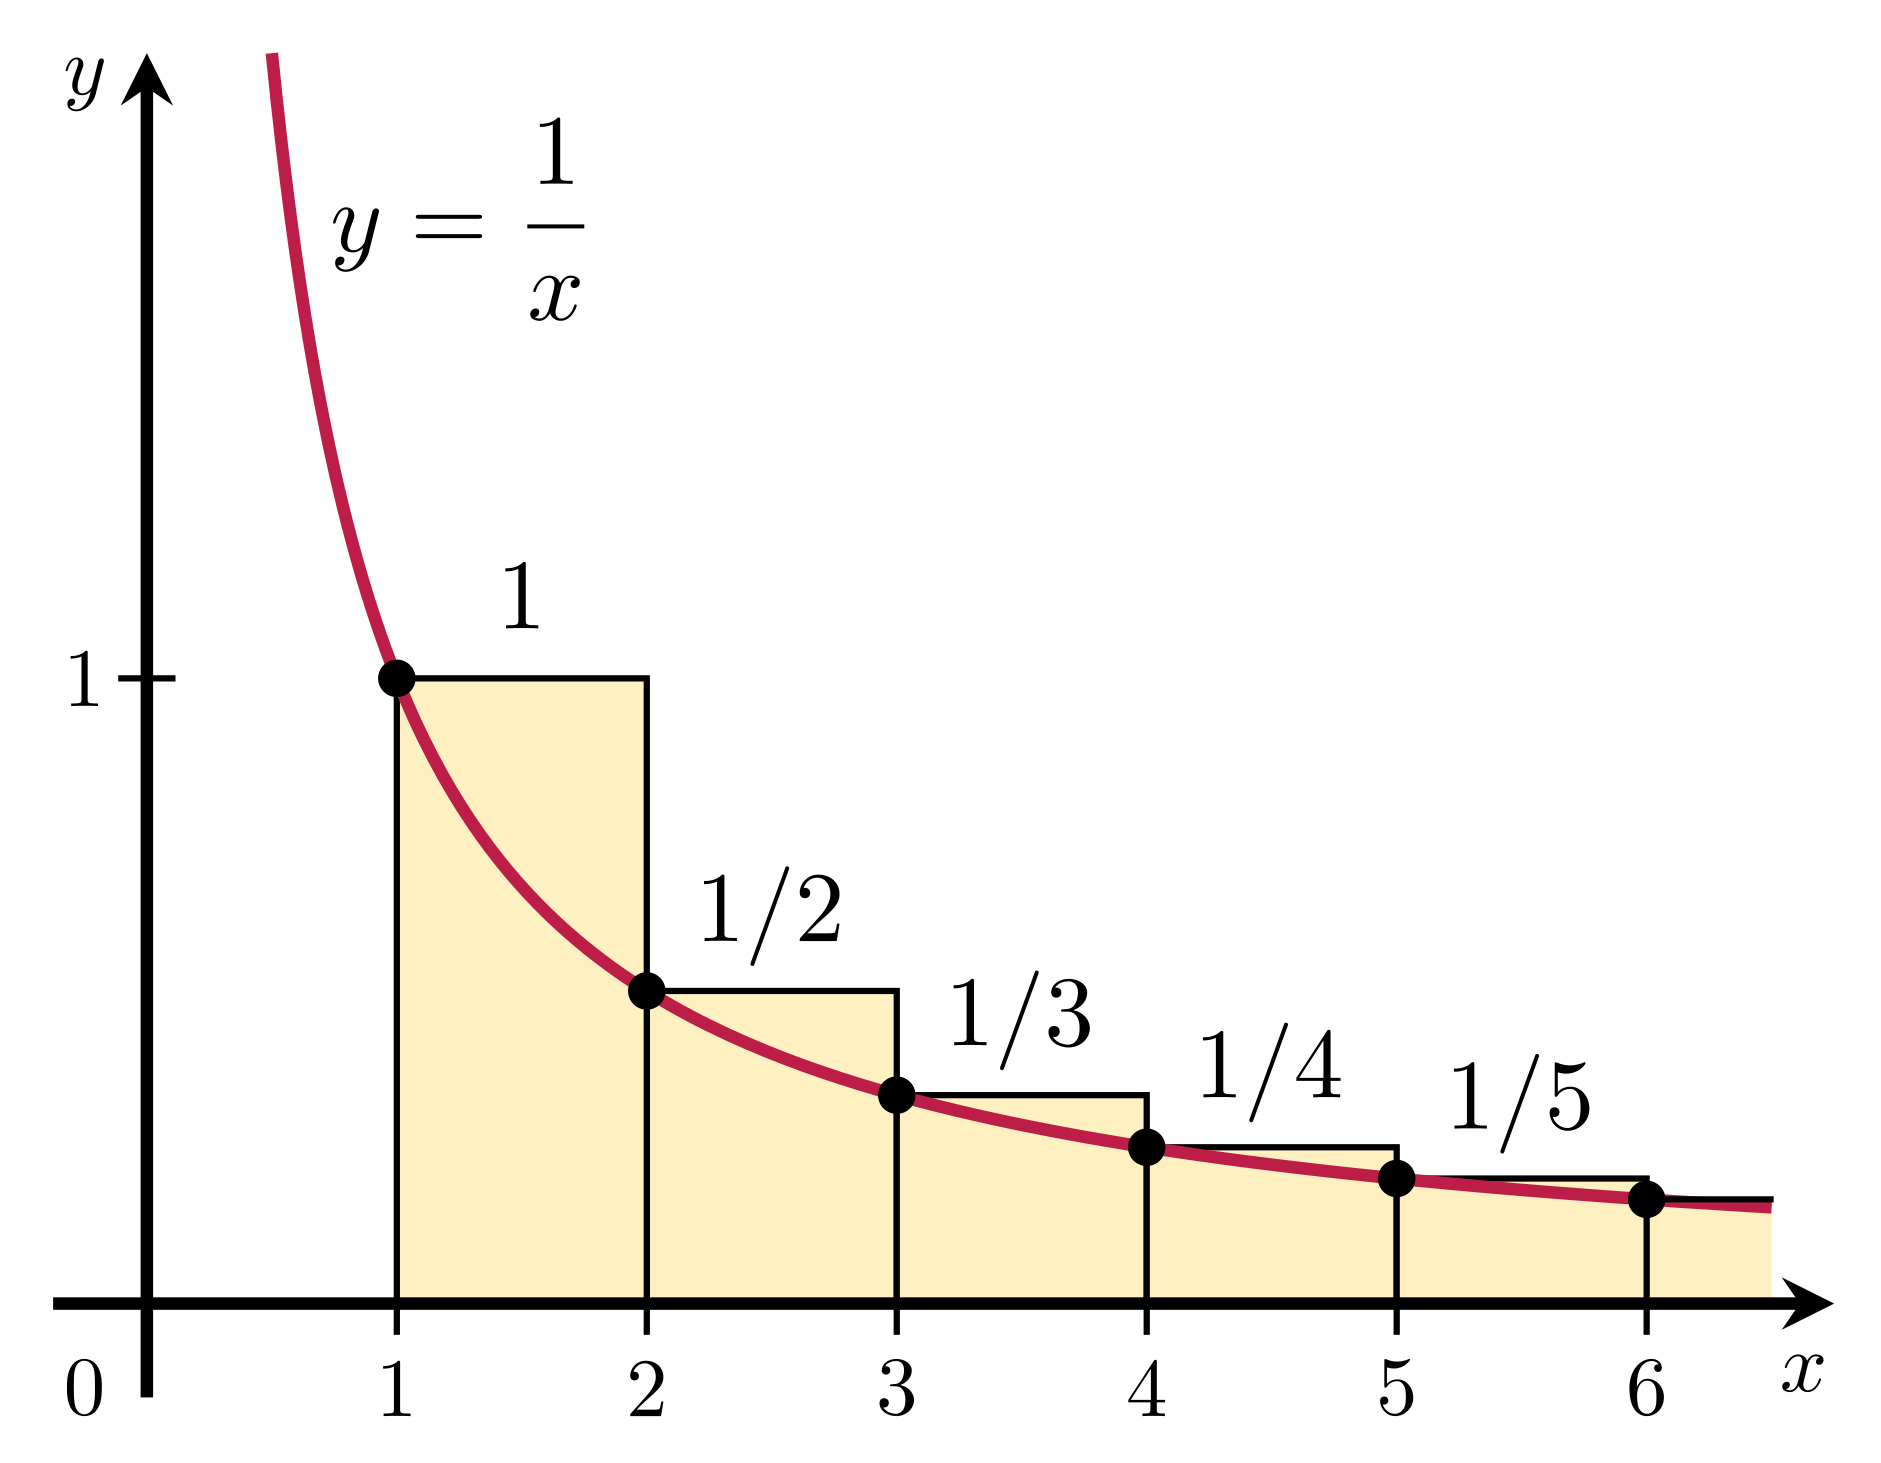
\includegraphics[width=10cm]{imagenes/Integral_Test.png}
    \caption{Los números armónicos están dados aproximadamente por el área bajo la hipérbola y, por lo tanto, pueden aproximarse mediante un logaritmo}
    \label{fig:gráfica de integrales}
\end{figure}

Lo que da como resultado una probabilidad de supervivencia asintótica dada por la ecuación \ref{eq:prob_supervivencia_n_resuelta}

\begin{equation}\label{eq:prob_supervivencia_n_resuelta}
    \begin{split}
        \lim_{n \to \infty} (1-H_2n+ H_n)&=1-\gamma+\gamma-\ln 2 \\
        &=1-\ln 2 \\
        &\approx0.30685
    \end{split} 
\end{equation}

Dado que la secuencia de probabilidades es monótonamente decreciente , los presos sobreviven con la estrategia de seguimiento del ciclo en más del 30\% de los casos independientemente del número de presos.